\documentclass{article}

% Language setting
% Replace `english' with e.g. `spanish' to change the document language
\usepackage[french]{babel}
\usepackage[fleqn]{amsmath} % Aligner les équations à gauche


% Set page size and margins
% Replace `letterpaper' with`a4paper' for UK/EU standard size
\usepackage[letterpaper,top=2cm,bottom=2cm,left=3cm,right=3cm,marginparwidth=1.75cm]{geometry}

% Useful packages

\usepackage{amsmath}
\usepackage{graphicx}
\usepackage{subcaption}
\usepackage[colorlinks=true, allcolors=blue]{hyperref}

\title{TD 10}
\author{IPESUP - PC }
\date{24/01/2024}

\begin{document}
\maketitle



\section{Naufrage d'un bateau}

On étudie un bateau qui coule dans la mer considérée comme un fluide parfait incompressible.
de masse volumique u. On note $H = 20 m$ la hauteur du bateau, $M = 50000$ tonnes sa masse
2 et $S = 8500 m^2$ sa surface de base :

\begin{figure}[h]
  \centering
  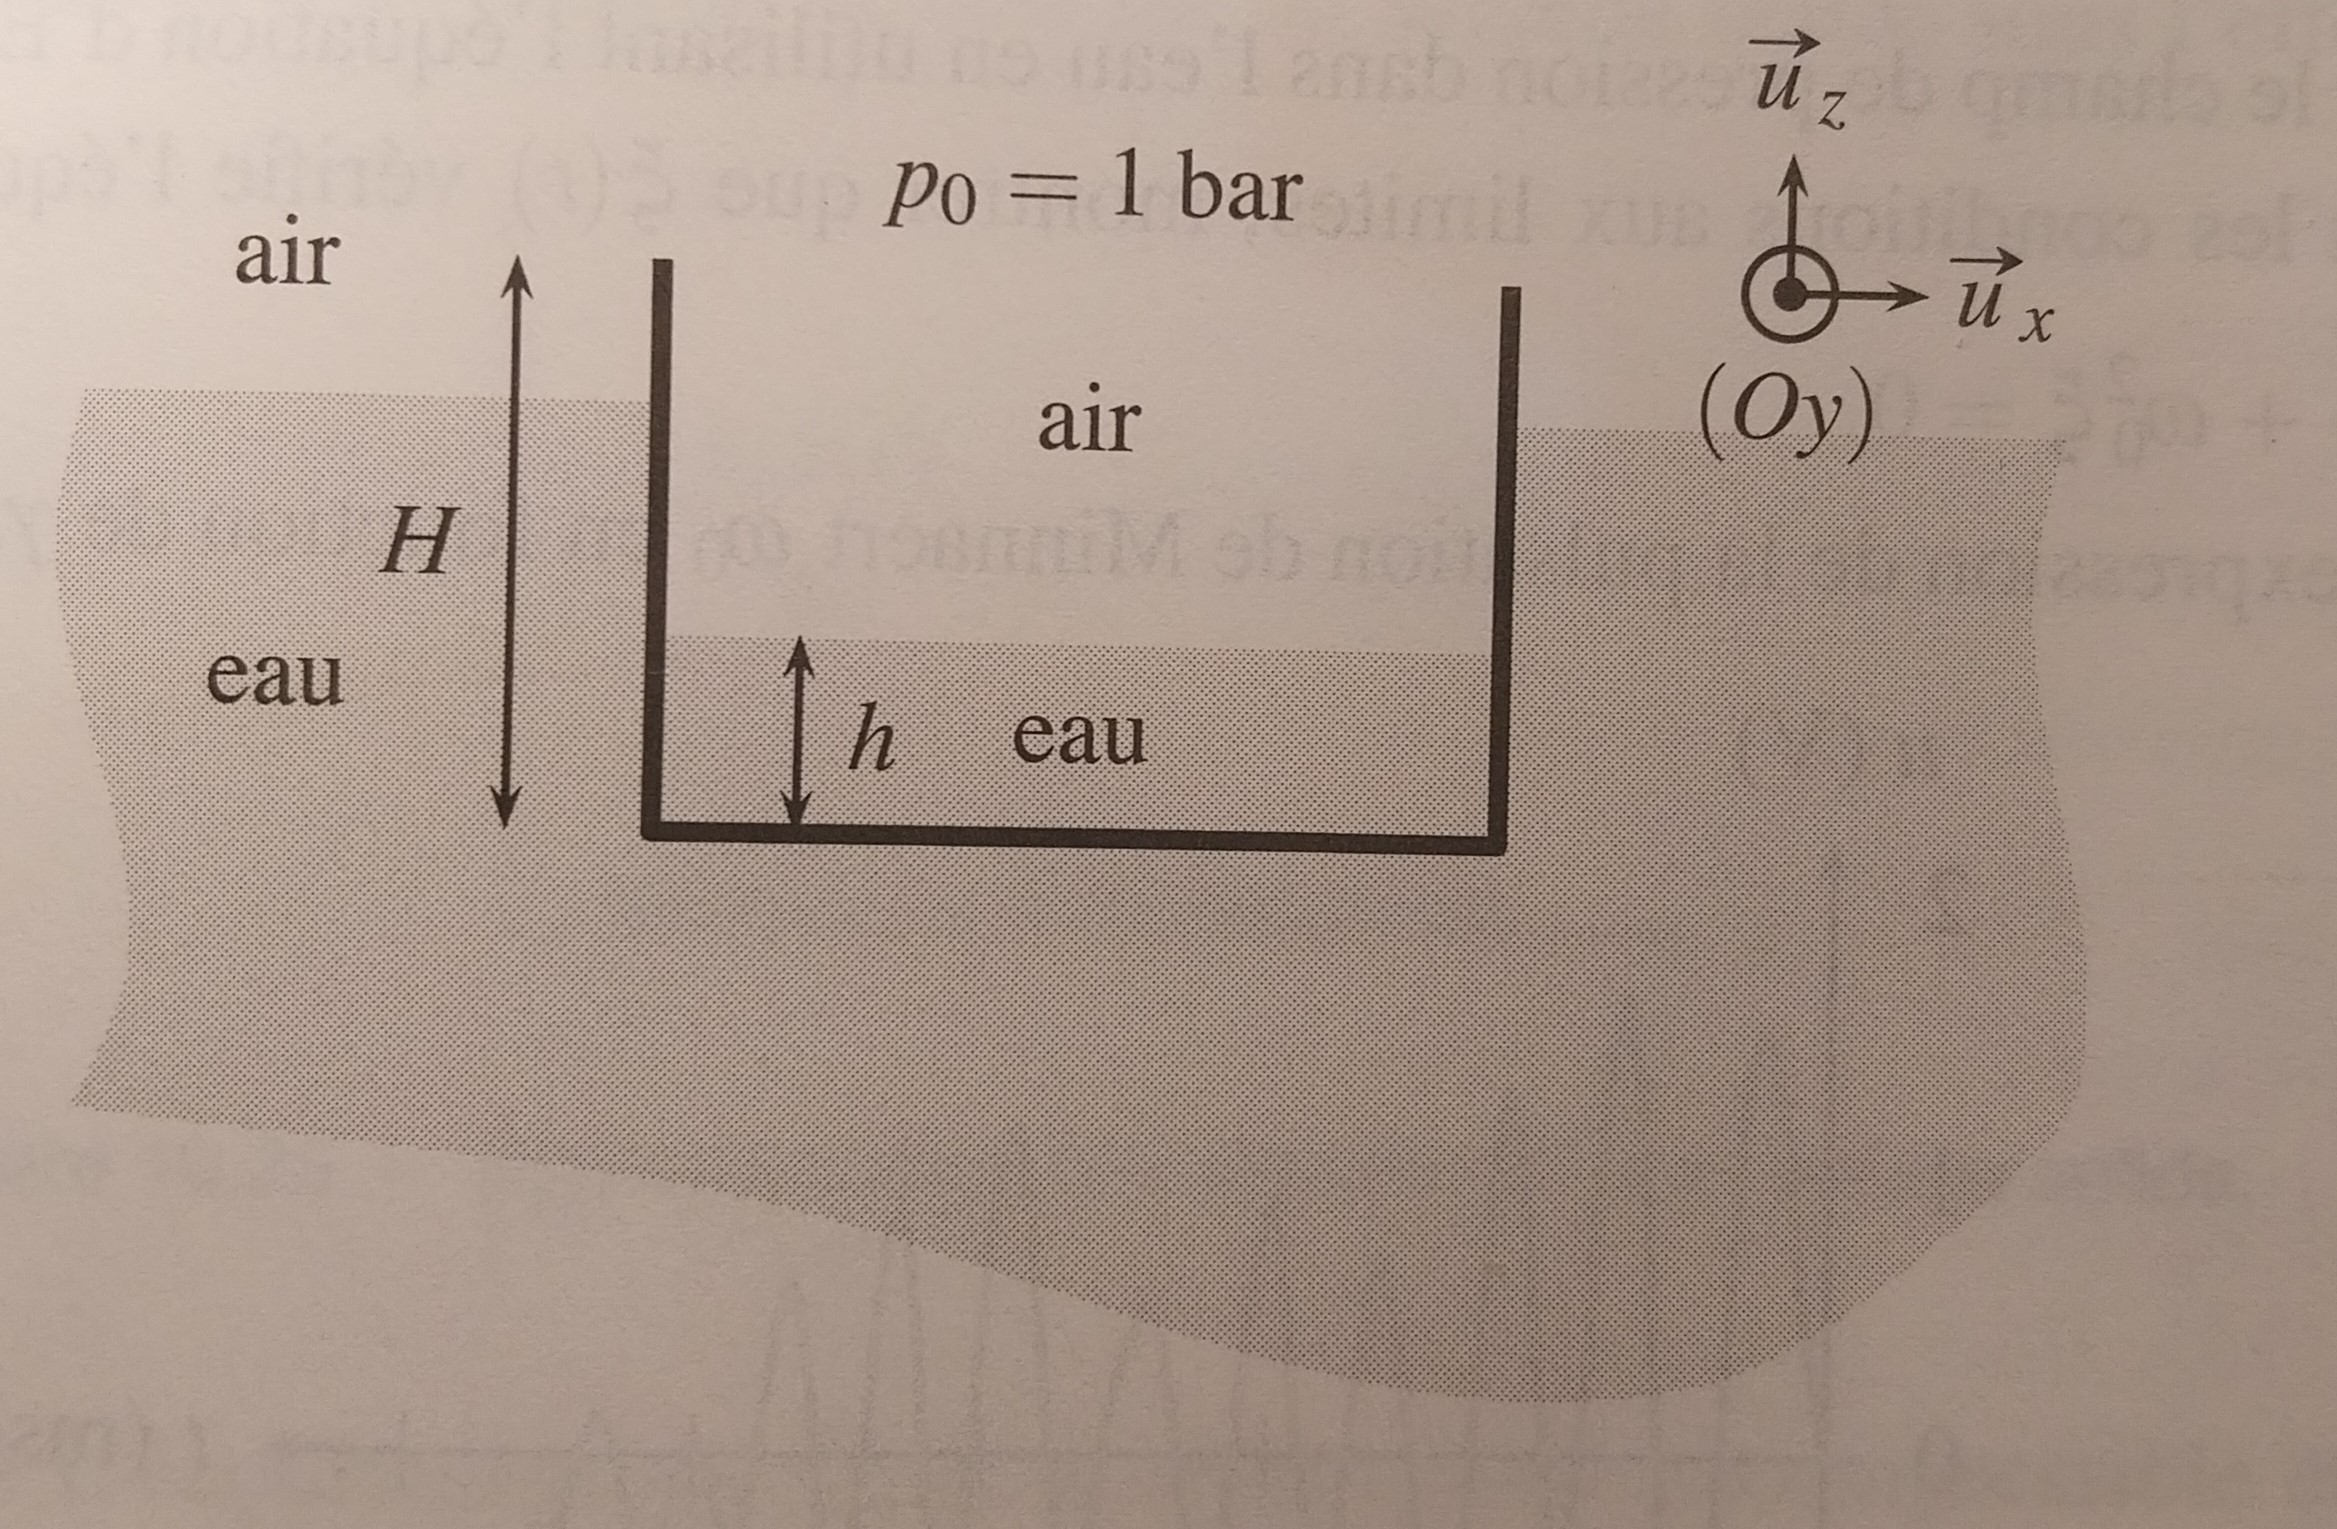
\includegraphics[width=0.4\textwidth]{naufrage_bateau.jpg}
  \label{fig:maison}
    \caption{Schéma du naufrage}
\end{figure}


\begin{enumerate}
 \item  On considère que le bateau est rempli d’eau sur une hauteur $h$. Quelle est la hauteur $h_m$, à
partir de laquelle le bateau coule ?
\item On considère maintenant que le bateau est initialement vide et qu'il se remplit par un petit
trou de surface $s << S$ situé dans la coque à une hauteur $l=4m$ du fond.
\begin{enumerate}
  \item Décrire les différentes étapes du remplissage.
  \item Déterminer $ h(t) $ pendant la première phase et caleuler sa durée $t_1$ .
  \item Déterminer $h(t)$ pour $t > t_1$.
  \item Quelle est la durée totale du naufrage ?
\end{enumerate}

\end{enumerate}


\section{Le chant des bulles:}


On considère une bulle d’air, assimilé à un gaz parfait de masse volumique $\mu_a$, sphérique,
de rayon $R_0$ et immergée dans un volume d’eau infini, homogène de masse volumique $\mu_0$. À
l’état de repos, la pression est uniforme et stationnaire ; sa valeur est notée $p_0$. 
À un instant $t=0$, la bulle d’air commence à « pulser » avec une amplitude faible. Son rayon
à un instant $t$ ultérieur est noté $R(t)=R_0 + \xi (t)$, avec $\xi << R_0$. On limitera tous les calculs
au premier ordre en $\xi / R_0$ . L’écoulement induit dans l’eau par les pulsations de la bulle
est supposé parfait et incompressible. On négligera tout écoulement d’air dans la bulle. On
admet que la symétrie sphérique de la bulle persiste au cours de son mouvement. En raison
du mouvement de la bulle, la pression $p(t)$ s’écarte de sa valeur de repos $P_0$. On supposera que la pression dans la bulle est uniforme. 


\begin{enumerate}
  \item On suppose que l’évolution de l’air contenu dans la bulle est adiabatique et réversible,
  On note $\gamma = \frac{C_p}{C_v}$ le coefficient isentropique de l’air, que l’on suppose indépendant de la
  température.
  Établir l’expression de la pression $p(t)$ en fonction de$P_0$, $\gamma$,  $R_0$ et $\xi(t)$.
  \item Justifier, grâce à des arguments de symétrie, que le champ de vitesse dans l’eau est de la
  forme : $\vec{v}(M,t)=v(r,t)\,\vec{u}_r$.
  \item En utilisant la propriété d’incompressibilité de l’écoulement, déterminer le champ de vitesse
  dans l’eau.
  \item Déterminer le champ de pression dans l’eau en utilisant l’équation d’Euler.
  \item En écrivant les conditions aux limites, montrer que $\xi(t)$ vérifie l’équation différentielle
  suivante : $:\frac{{\mathrm{d}}^{2}\xi}{{\mathrm{d}t}^{2}}+{\omega}_{0}^{2}\xi=0.$
  On donnera l’expression de la pulsation de Minnaert $\omega_0$ en fonction de $\gamma, p_0, \mu_0 $ et $ R_0$

  \begin{figure}[h]
    \centering
    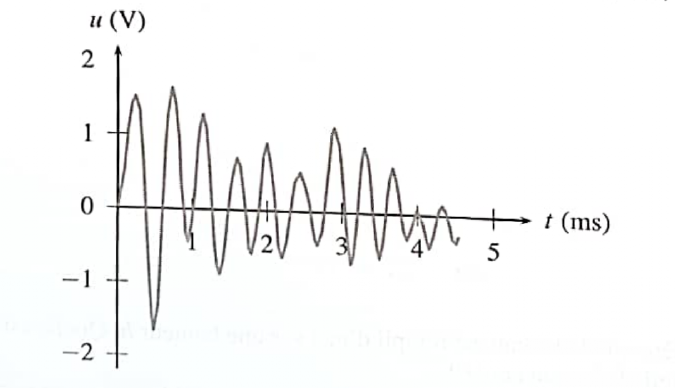
\includegraphics[width=0.4\textwidth]{bulles.png}
    \caption{Signal délivré par le microphone immergé}
    \label{fig:bulles}
  \end{figure}
  
  % Insert a reference to the previous figure:
  \item À l’aide d’un bulleur d’aquarium, on produit des bulles d’air dans un récipient rempli
    d’eau. Un microphone immergé « écoute » les vibrations des bulles formées. Le signal délivré
    par le microphone est représenté sur la figure 2. En déduire une estimation du rayon des
    bulles formées.

\end{enumerate}
  
\section{Eolienne}

  On cherche à déterminer la puissance prélevée au vent par le rotor d’une éolienne. En amont,
loin de l’éolienne, le vent est uniforme et permanent de vitesse $\vec{v_0} = v_0 \vec{u_x}$ , et la pression
est uniforme et vaut $P_0$. On néglige les effets de la pesanteur. L'éolienne est formée d’un mât, dont on négligera
 l’influence, portant un rotor d’axe horizontal que l’on assimilera à un
disque de diamètre $D$ et de surface $S_0$. 
L’écoulement de l’air est unidimensionnel, stationnaire, incompressible et parfait. La masse volumique de l’air est notée $\mu$ .
La figure suivante représente l’allure du tube de courant s’appuyant sur le pourtour du rotor,
les valeurs de la pression et de la vitesse sont précisées sur la figure 3.

\begin{figure}[h]
  \centering
  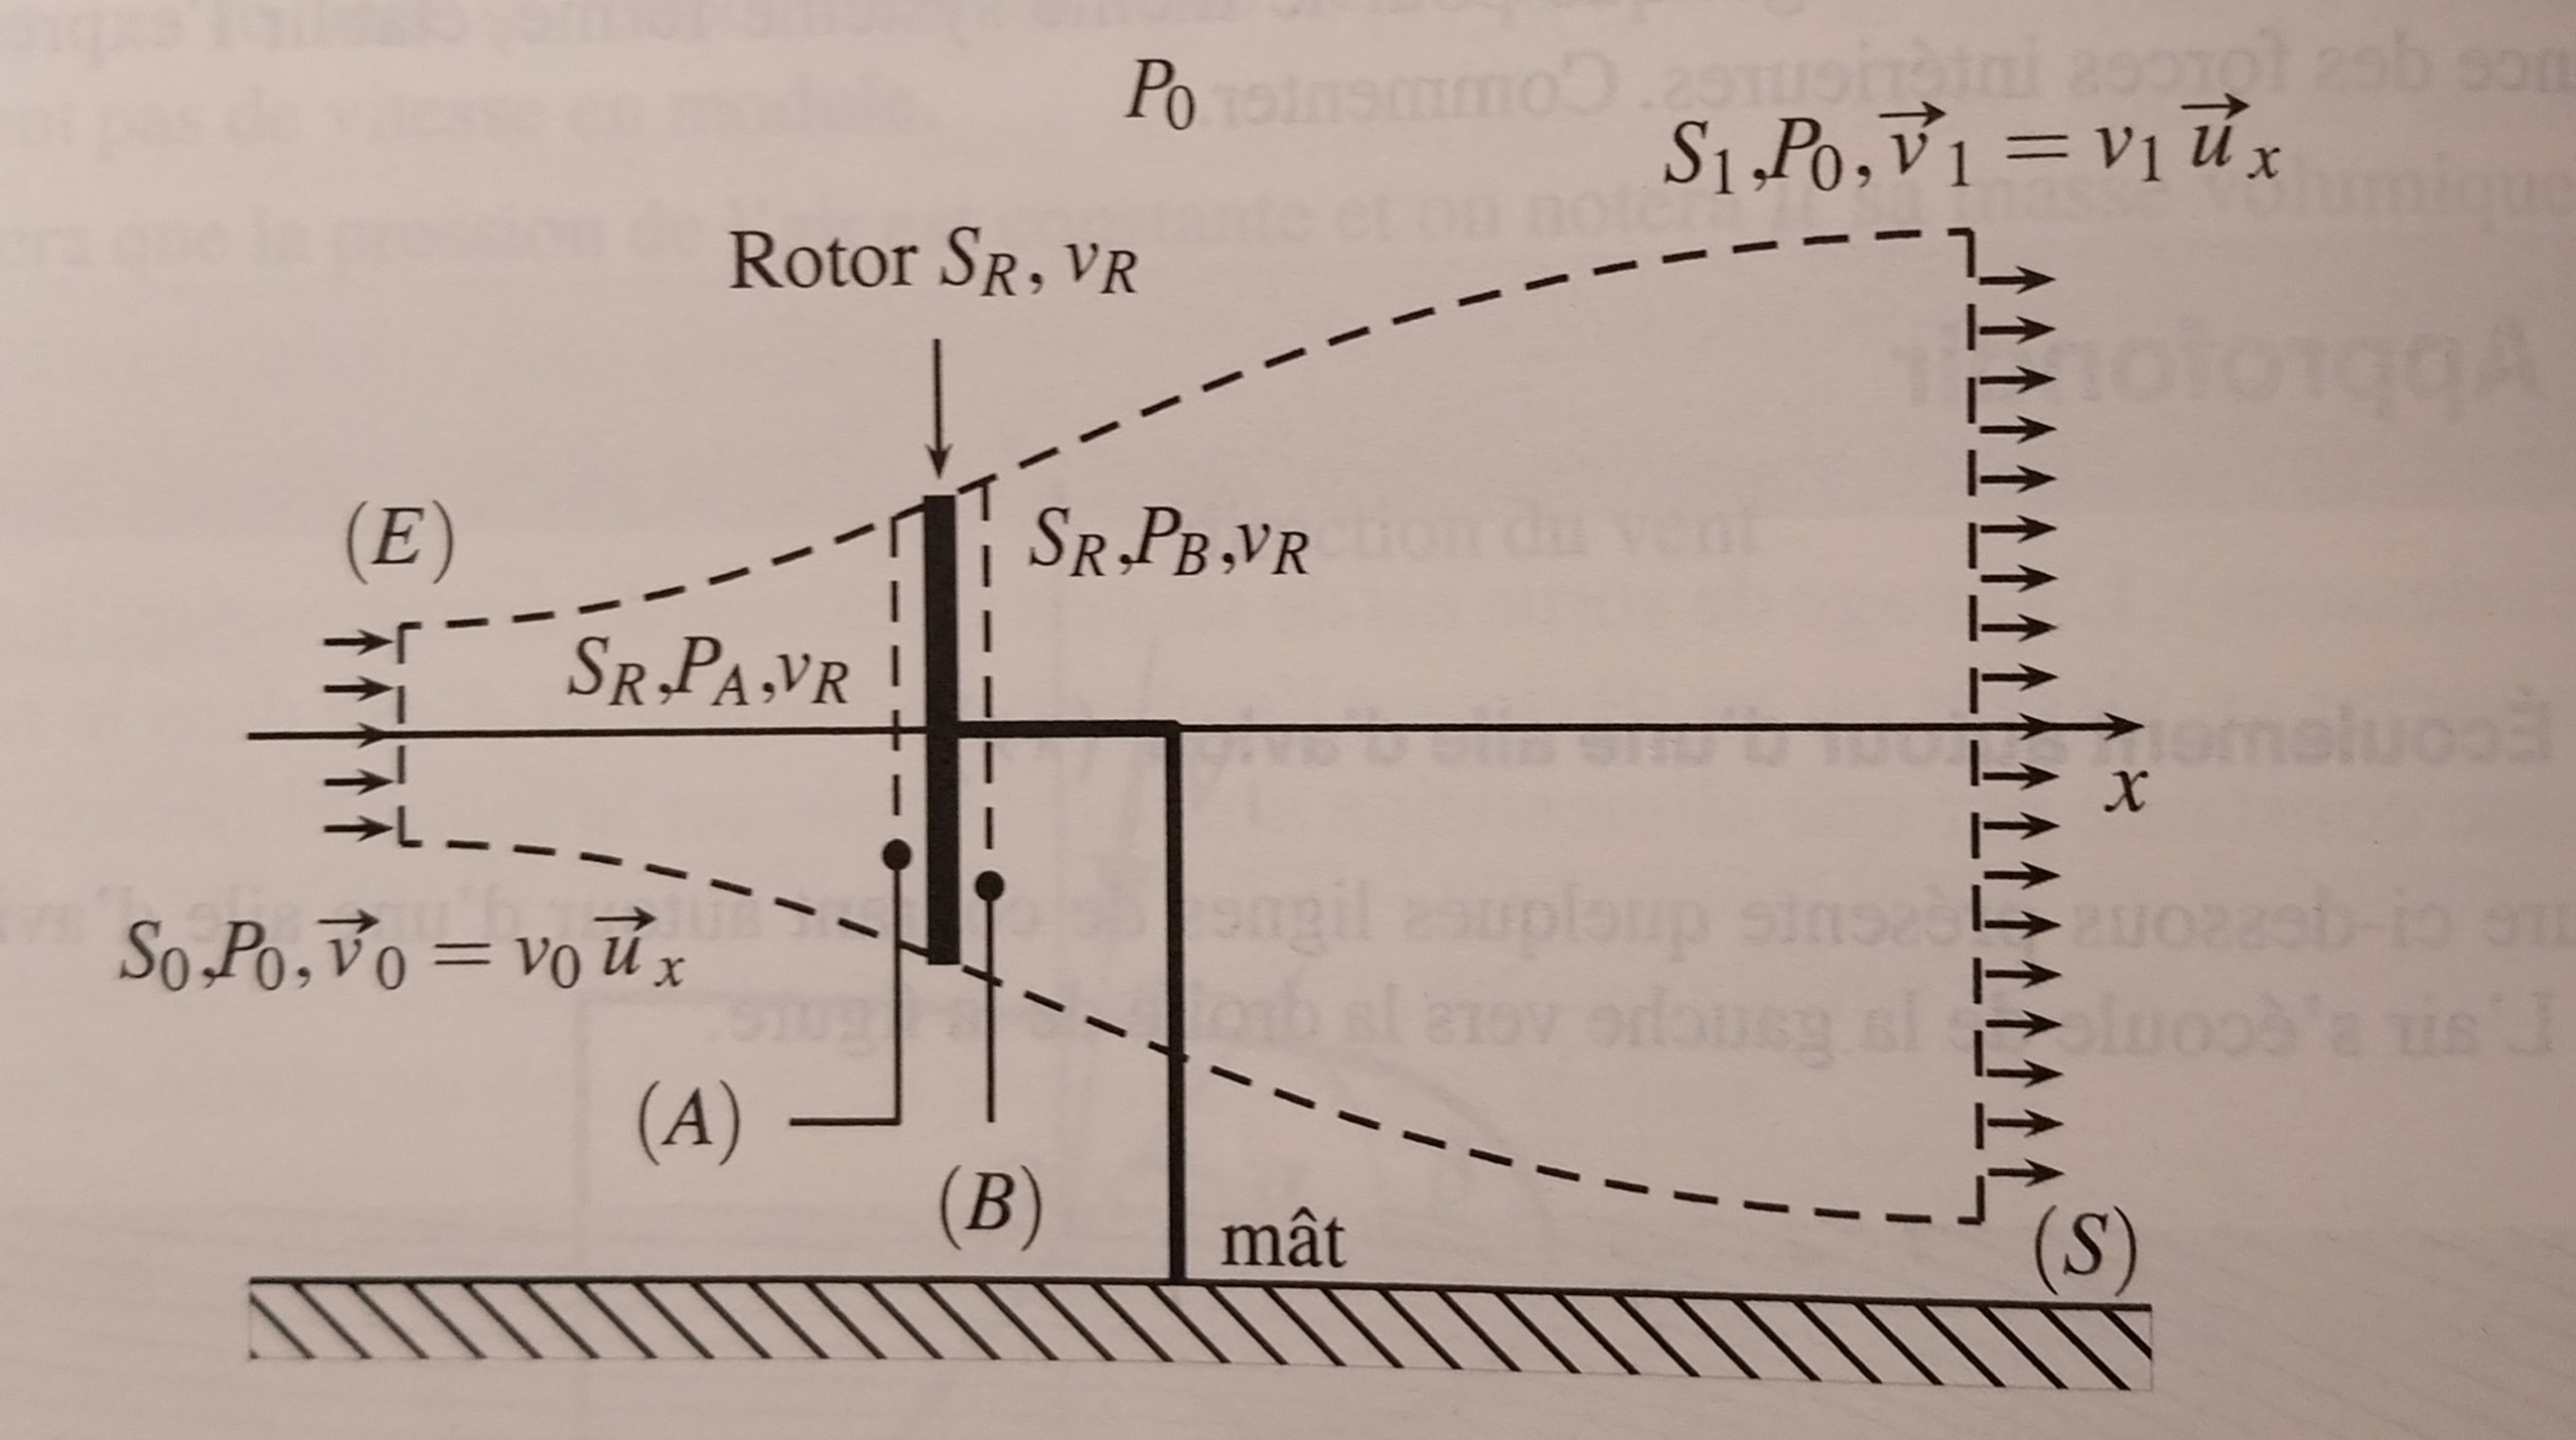
\includegraphics[width=0.55\textwidth]{éolienne.jpg}
  \caption{Eolienne}
  \label{fig:eolienne}
\end{figure}

Les surfaces $(A)$ et $(B)$ sont situées de part et d’autre du rotor à proximité immédiate et on
prend donc : $S_A = S_B = S_R$ et $\vec{v}_{A}=\vec{v}_{B}=\vec{v_R}=v_{R}\vec{u}_{x}$. 
On désigne par $\vec{F} = F\vec{u_x}$ la force
totale exercée par l’hélice sur le fluide.
\begin{enumerate}
  \item Étant donné l’allure du tube de courant, que peut-on dire de $v$ et de $v_0$ ?
  \item En faisant un bilan de quantité de mouvement sur un système que l’on précisera, établir
  une relation liant $v_0, v_1, S_0, \mu et F $. 
  \item  En faisant un bilan de quantité de mouvement, établir une relation liant $P_A$,$  P_B$, $S_R$ et $F$. En
  déduire l’expression de la vitesse de l’air au niveau du rotor $v_r$ en fonction de $v_0$ et $v_1$.
  \item Déterminer, à partir d’un bilan énergétique, l’expression de la puissance $\mathcal{P}$ des actions
  mécaniques que le vent exerce sur le rotor en fonction de $\mu$, $S_R$, $v_0$ et du rapport $\alpha = v_1/v_0$.
  Pour quelle valeur de $\alpha$ cette puissance est-elle maximale ? Exprimer $\mathcal{P}$  en fonction de $\mu$, $S_r$ et $v_0$. 
\end{enumerate}

\section{Le mascaret de Gironde}

Lorsque la marée commence à monter, l’eau de l’océan s’engouffre dans l’estuaire de la
Gironde. Le flux de la marée se heurte alors au courant du fleuve et une série de vagues se
forment. Elles constituent ce qu’on appelle un mascaret, qui grossit au fur et à mesure de  sa
progression et sa hauteur peut atteindre jusqu’à deux mètres de haut. Cette série de 5 à 10
vagues rapprochées se déplace à une vitesse de 15 à 30 km/h ,et remonte ainsi le fleuve sur
près de 200 km à l’intérieur des terres.
On modélise le fleuve par un canal horizontal d’axe (Ox), de profondeur constante $L$ selon
(Oy). En amont de la vague, le fleuve s’écoule à la vitesse $\vec{v_1} = u \vec{u_x}$ et de hauteur $h_1$.
Le mascaret est modélisé par une marche : en aval du front de la vague, la hauteur d'’eau
est $h_2>h_1$. La hauteur du mascaret est donc $H = h_2 - h_1 > 0$. On admet que le mascaret se déplace à vitesse constante 
$-c\vec{u_x}$ dans le sens des x décroissants. Partout, l'écoulement ests upposé incompressible et le fluide homogène, de masse 
volumique $\mu$. On note $p_1(M)$ et $p_2(M)$ les champs de pression dans les écoulements en amont et en aval du mascaret. 
On suppose la pression dans l'air uniforme égale à $p_0$.On se place dans le référentiel du mascaret, galiléen, dans lequel
l'écoulement est stationnaire avec des vitesses $\vec{v_1'} = (c+u)\vec{u_x}$ et $\vec{v_2'}$ en amont et en aval du mascaret. 
\begin{figure}[h]
  \centering
  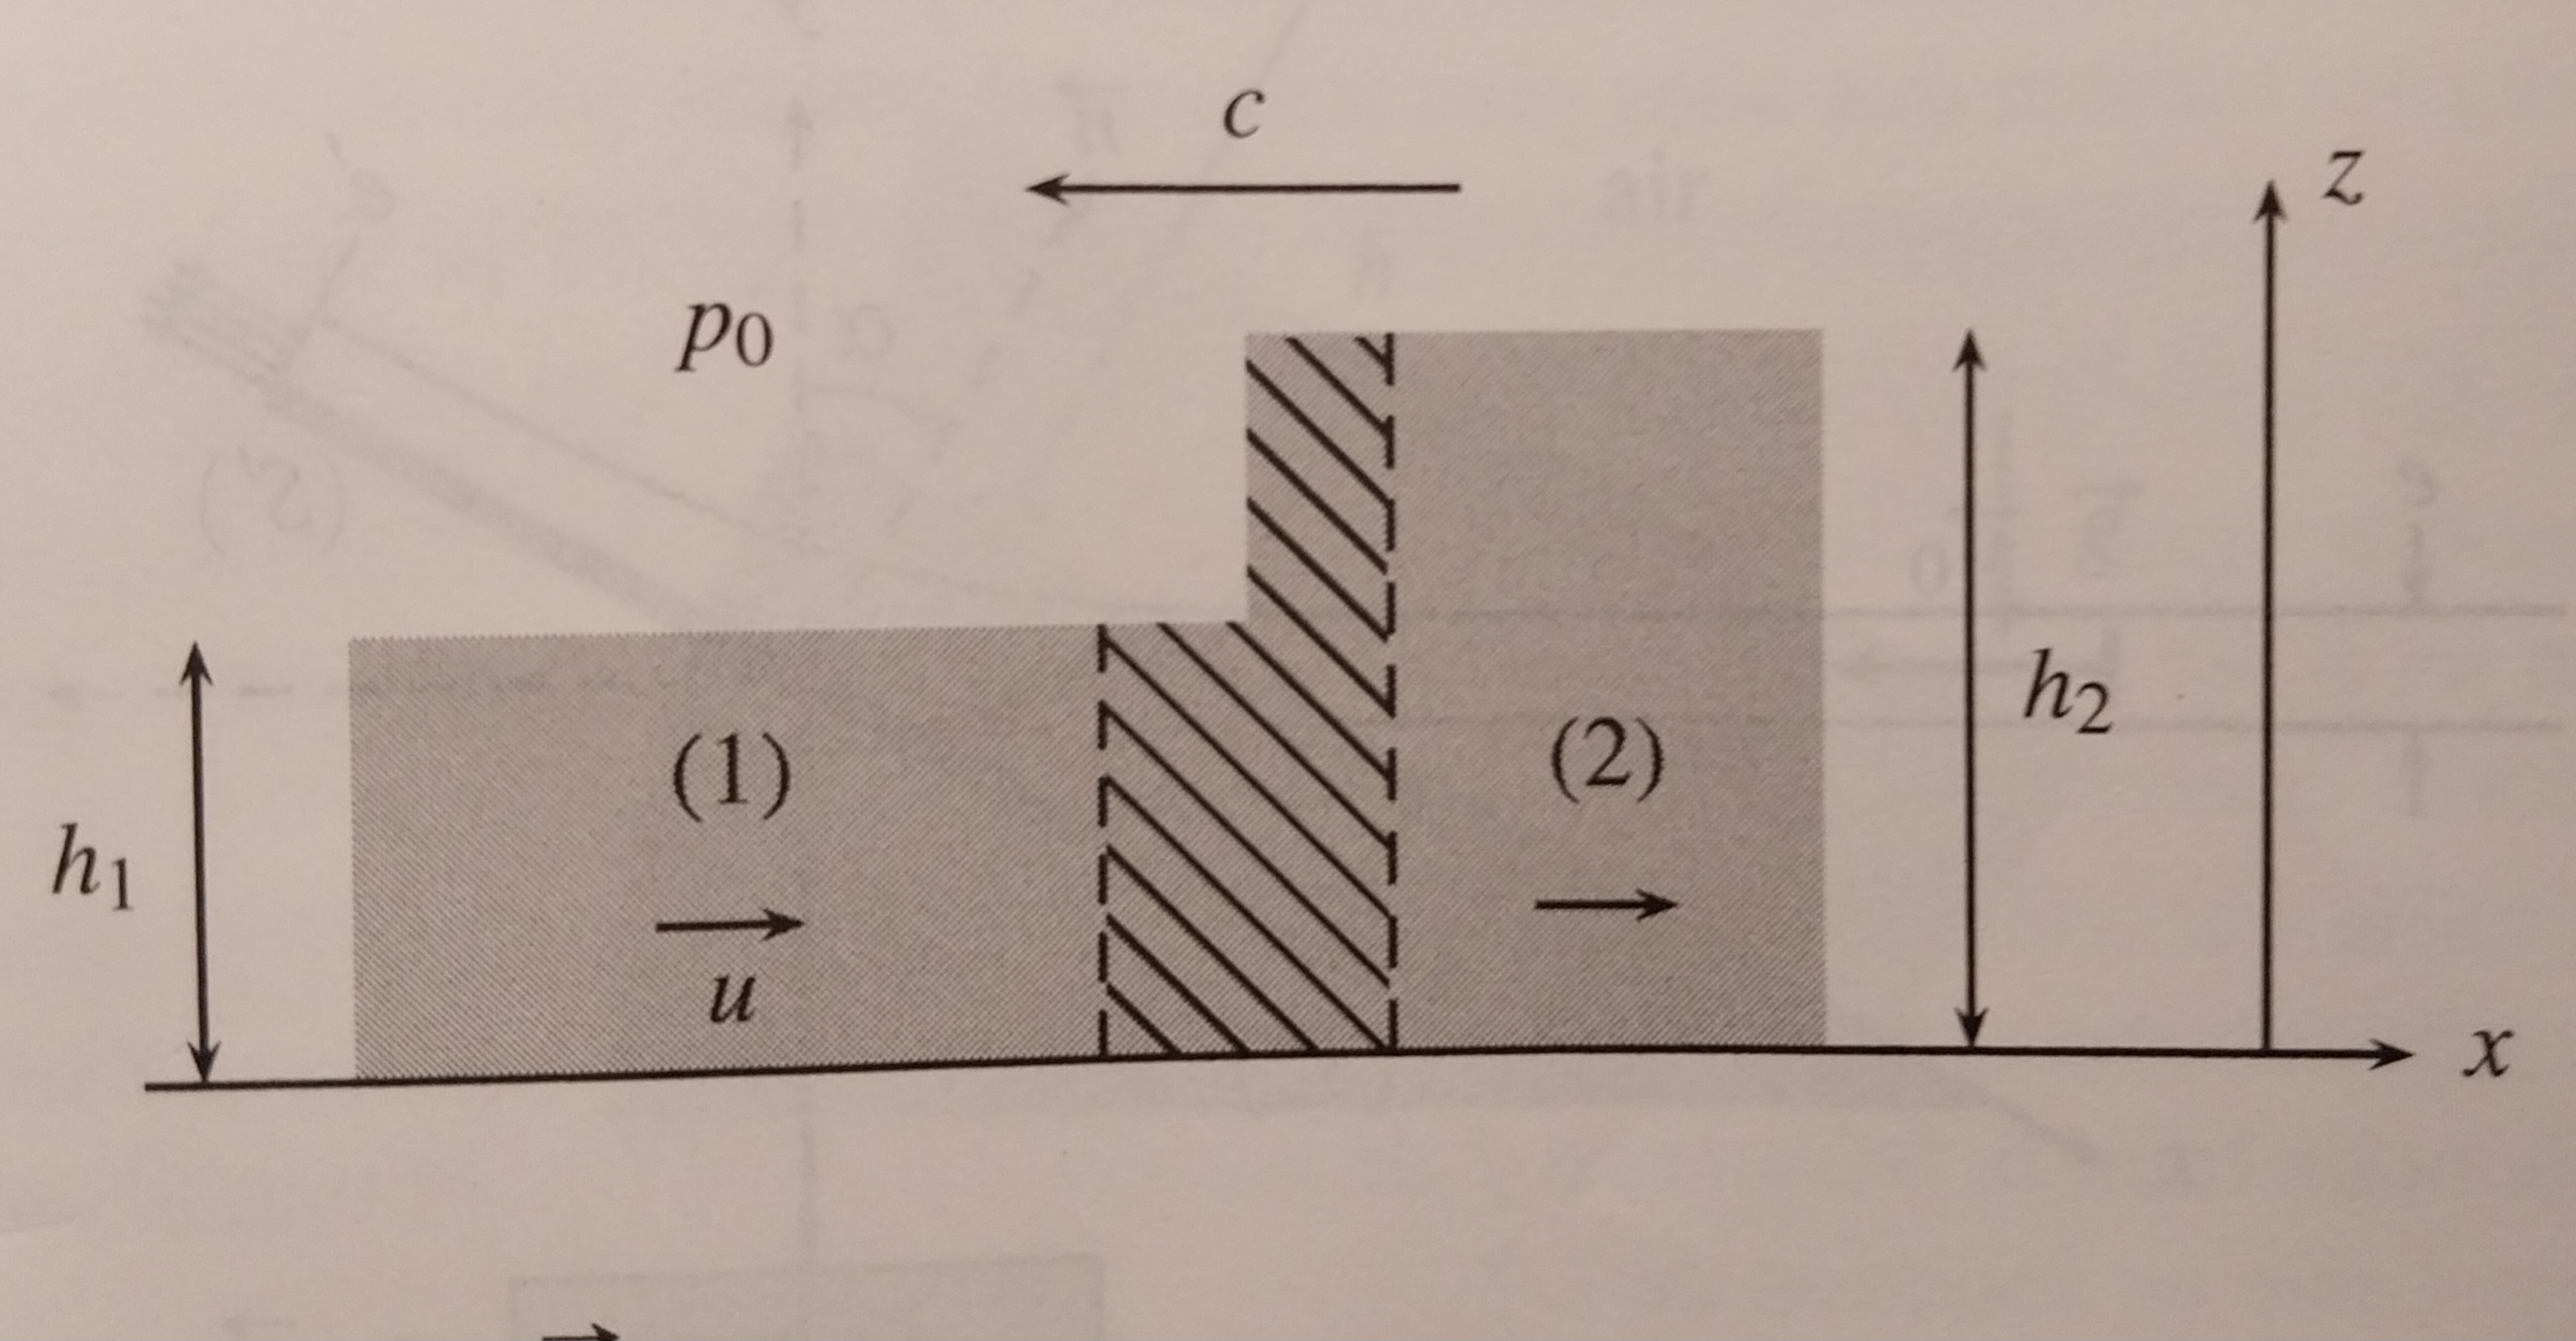
\includegraphics[width=0.55\textwidth]{gironde.jpg}
  \caption{Mascaret}
  \label{fig:mascaret}
\end{figure}
\begin{enumerate}
  \item Justifier l’expression de $\vec{v_1'}$ .
  \item En faisant un bilan de masse, déterminer la vitesse $\vec{v_2'}$.
  \item Justifier que dans chacun des écoulements en amont et en aval du mascaret, la distribution
  de pression est hydrostatique.
\item On considère le système ouvert constitué de l’eau contenue à l’instant $t$ dans le volume
  hachuré sur la figure. Montrer que la résultante des forces de pression exercées par l’eau sur
  ce système est la somme de la résultante des forces de pression $\vec{F_{p1}}$ s’exerçant sur la hauteur
  $h_1$,et $\vec{F_{p2}}$ s’exerçant sur la hauteur $h_2$ :
  \\[0.1cm]



  $\vec{F}_{p1}=\left(p_{0}L h_{1}+\frac{1}{2}\mu g L h_{1}^{2}\right)\overrightarrow{u}_{x}\,\mathrm{et}\,\overrightarrow{F}_{p2}=-\left(p_{0}L h_{2}+\frac{1}{2}\mu g L h_{2}^{2}\right)\overrightarrow{u}_{x}\,.$


  \\[0.1cm]



\item En admettant qu'on peut négliger la viscosité et en faisant un bilan de quantité de mouvement, montrer que: 


\\ 

$(c+u)^{2}={\frac{1}{2}}g{\frac{h_{2}}{h_{1}}}(h_{1}+h_{2})\,$

\item On se place dans la situation où $h_1 = 10,0m$ et $h_2 = 12,0 m$. 
À quelle condition sur la valeur de $u$, le mascaret parvient-il à remonter le fleuve ?

\end{enumerate}
\end{document}

